\doublespacing
\chapter{Literature Review} \label{chap:literatureReview}

%\version{v1.10.2015}


From the past few years Pakistan has been facing the problems of food wastage. About quoter of food that is being produced in the country is wasted. The country has majority of the people that are living in food insecurities and many of the population can not provide proper food to their families \cite{wenlock1980household}. On the other hand the stats for food wastage is high in the country and it is growing day by day. So the situation is not balance out. The production companies are contributing the most in terms of food wastage and their products gets expired so they have to throw away their expired products which produces the waste \cite{zhao2022exploring}. These companies face huge losses as their products gets expired. The hotels and marquees also faces the problem of excessive food being wasted on events and marriages. Seeing all this above problems what we have  proposed the solution that is, if a company has products or food items that are near to expiry date than they will place their product on bidding through our web application and the bid price should be as low as possible. So people will bid on the product and the one with the highest bid will will the bid. So, in this way we created a win win situation for both the buyer and seller.
\section{Previous Work}
There are the application that are already in this domain and the details of these application are following:
\subsection{Too Good To Go}
The application Too Good To Go \cite{ref5} is only for the food donation, and it only covers the surplus food, as shown in Figure \ref{fig1}. They are unable to cover the vast area of food wastage. This application does not have transparency as you must login in order to see what the application has to offer. This is a mobile application.\\
\begin{figure}[!h]
    \centering
    \includegraphics[width=\linewidth, keepaspectratio ]{projectReportTemplate/figures/Tgtg.png}
    \caption{Too Good To Go }
    \label{fig1}
\end{figure}

\newpage
\subsection{OLIO}
Olio \cite{ref6} is a mobile application as shown in Figure \ref{fig olio}. Olio provides a platform for neighbours to share unwanted food and other items, all for free. They are unable to cover the vast area of food wastage. This application does not have transparency as you must login in order to see what the application has to offer. It also covers less working radius.\\
\begin{figure}[!h]
    \centering
    \includegraphics[width=\linewidth, keepaspectratio ]{projectReportTemplate/figures/Olio.png}
    \caption{OLIO}
    \label{fig olio}
\end{figure}
\newpage
\subsection{Karma}
Karma \cite{ref7} as shown in Figure \ref{fig karma} is a mobile application. It connects user from nearby grocery store through mobile application. The grocery store will notify if they have any surplus food available. If so, then they will gave it to users on low price.\\
\begin{figure}[!h]
    \centering
    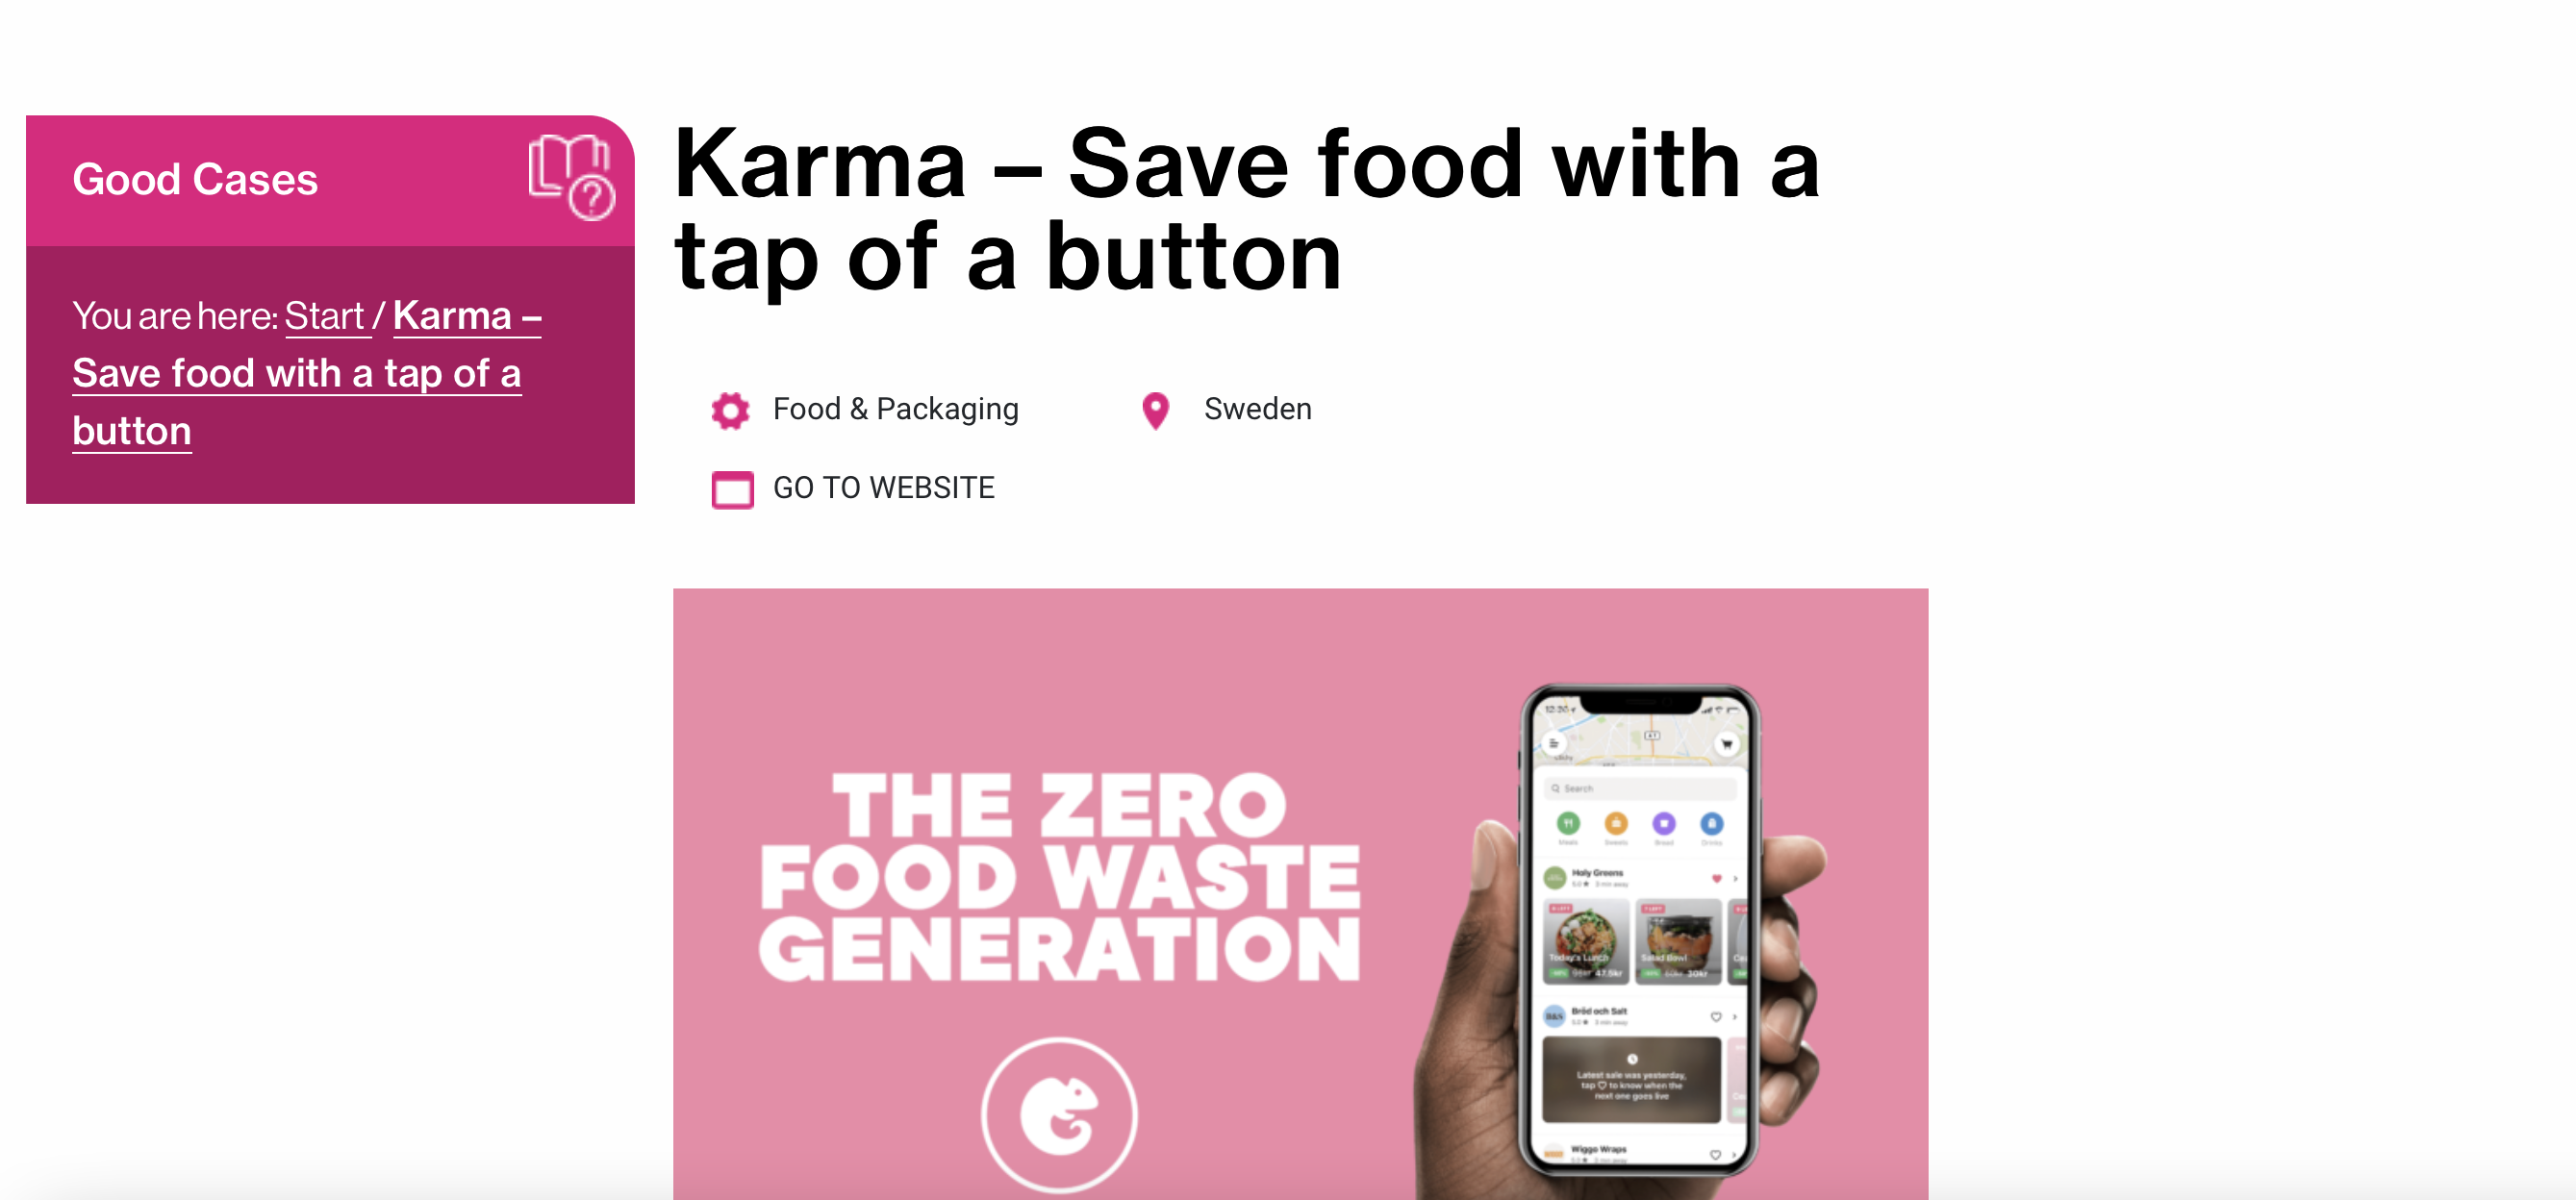
\includegraphics[width=\linewidth,keepaspectratio ]{projectReportTemplate/figures/Karma.png}
    \caption{Karma}
    \label{fig karma}
\end{figure}
\newpage
\subsection{Phenix}
Phenix as shown in Figure \ref{fig pheoinx} is a mobile application. This application helps the users to find the unsold items in nearby store. The products that are not sold for specific time frame will be listed to application so that people near the store can buy these products and help them reduce food waste.\\
\begin{figure}[!h]
    \centering
    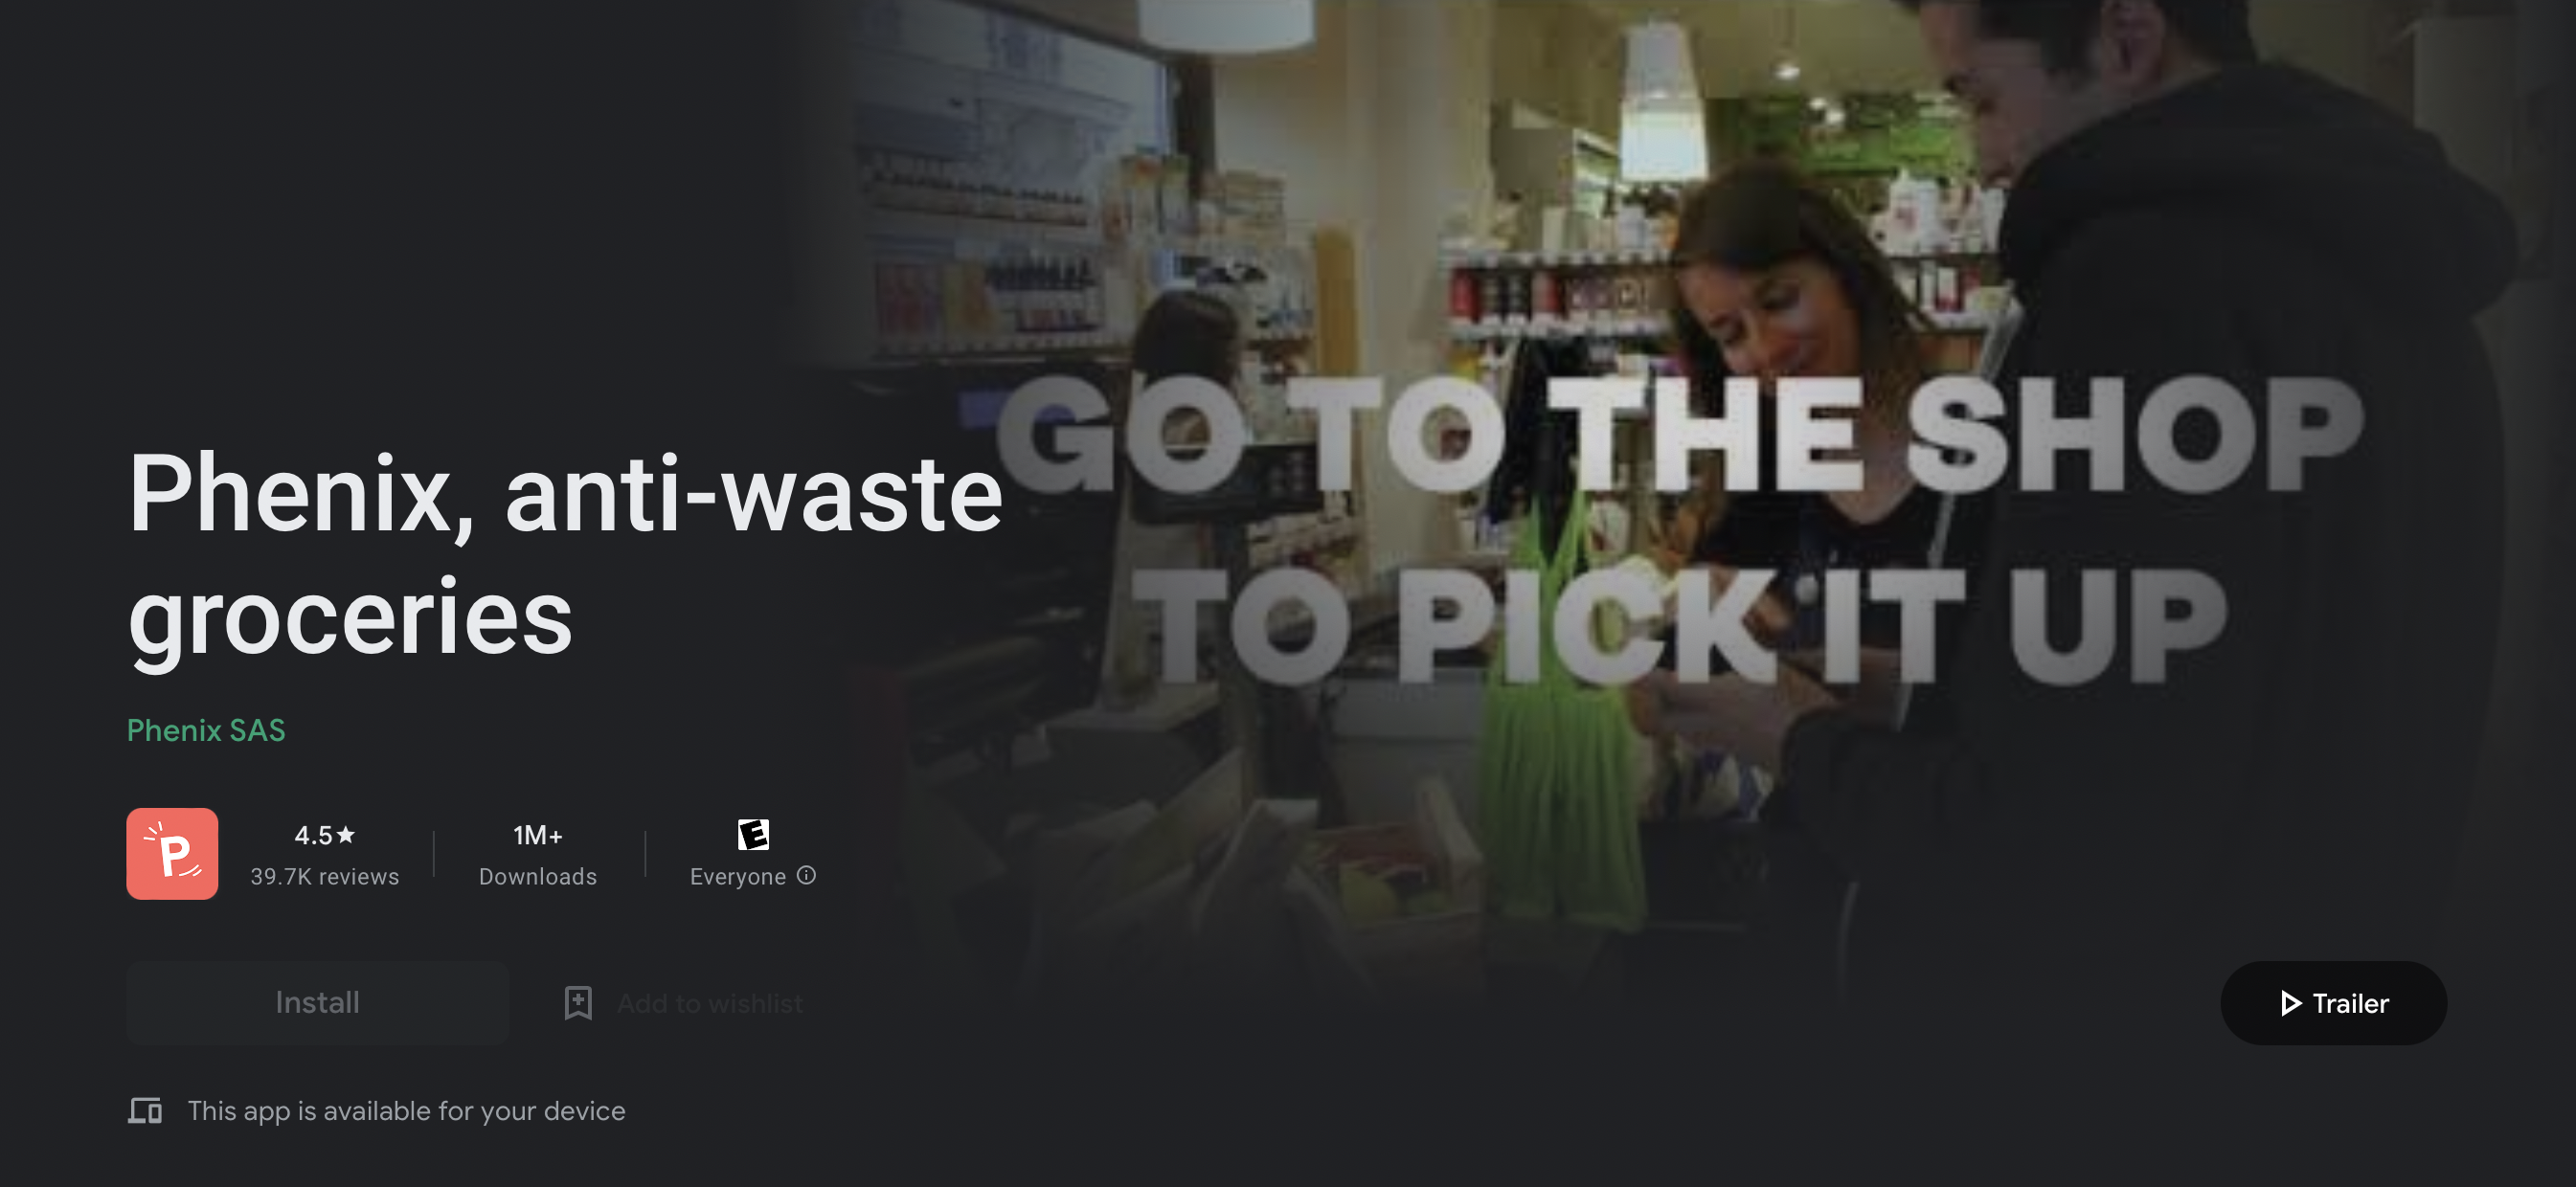
\includegraphics[width=\linewidth,keepaspectratio ]{projectReportTemplate/figures/Phenix.png}
    \caption{Pheonix}
    \label{fig pheoinx}
\end{figure}
\newpage
\subsection{FoodHero}
FoodHero \cite{ref8} as shown in Figure \ref{fig:Foodhero} is mobile appliaction. This application allow users to find food in their local area at lowest price as possilbe. The user simply add the discounted excess food in his cart and then he buys it from store to reduce the excess food wastage.\\
\begin{figure}[!h]
    \centering
    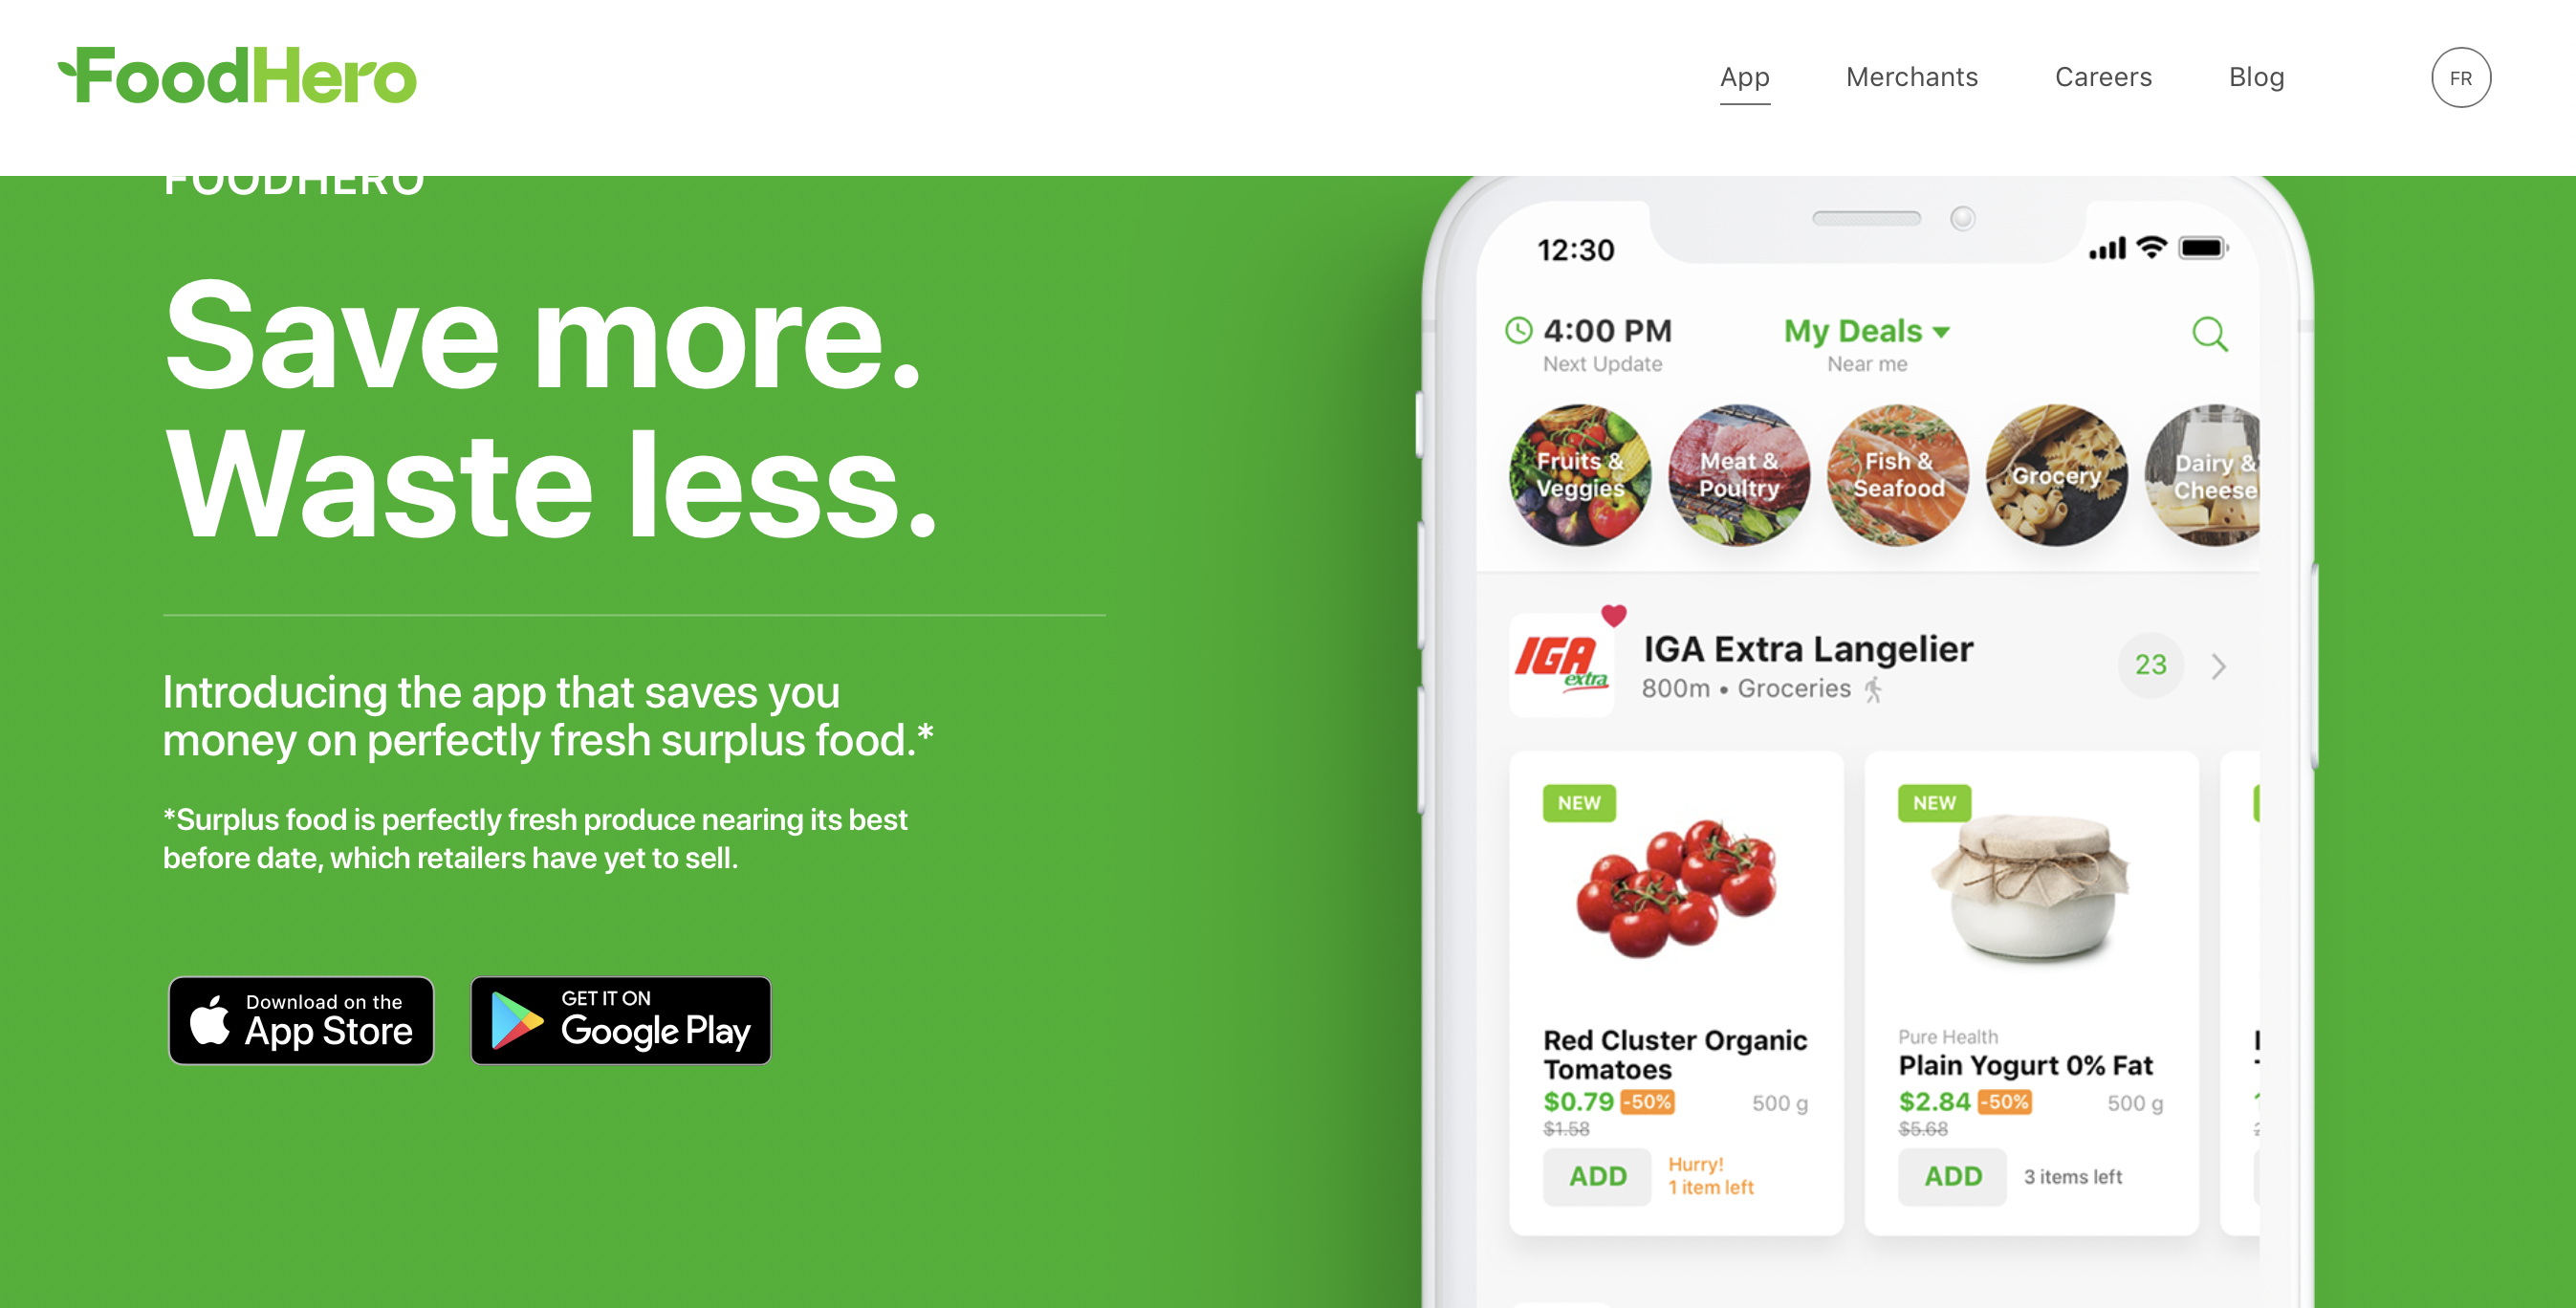
\includegraphics[width=\linewidth, keepaspectratio ]{projectReportTemplate/figures/FoodHero.png}
    \caption{FoodHero }
    \label{fig:Foodhero}
\end{figure}
\newpage
\section{Comparison Table}
The feature Table \ref{tab1} shows the comparison between our web application and our competitor in the same space. The competitor applications shown in the table are mobile base applications. Most of these applications works on free food and donation of food items while, proposed web application works on food bidding. These applications are restricted to mobile users only and the information about the food is only provided when we logged in to the system. Our proposed system provides data transparency and information about food without registration. \\
\begin{table}[!h]
    \centering
    \begin{tabularx}{1\textwidth} { 
  | >{\centering\arraybackslash}X 
  | >{\centering\arraybackslash}X 
  | >{\centering\arraybackslash}X 
  | >{\centering\arraybackslash}X 
  | >{\centering\arraybackslash}X 
  | >{\centering\arraybackslash}X 
  | >{\centering\arraybackslash}X |}
 \hline
 Comparison Table & Too Good To Goo & Olio & Karma & Phenix & Food Hero & Our Web Application\\
 
 \hline
 
 Data Transparency  & $\times$  & $\times$ & $\times$ & $\times$ & $\times$ & \checkmark{} \\

\hline

Bidding System  & $\times$  & $\times$ & $\times$ & $\times$ & $\times$ & \checkmark{}\\

\hline

Use on Mobile  & \checkmark{}  & \checkmark{} & \checkmark{} & \checkmark{} & \checkmark{} & \checkmark{}\\

\hline

Use on Web Browser  & $\times$  & $\times$ & $\times$ & $\times$ & $\times$ & \checkmark{}\\

\hline

\end{tabularx}
    \caption{Feature Table}
    \label{tab1}
\end{table}
 